\chapter{Models, Consistency and Processes
    \pgsize{15 p.}
}
\label{chap:networks}


%%
%% CONSISTENCY NOTIONS
%%
\section{Consistency Notions and Preservation}
\label{chap:networks:notions:normative_descriptive}

In the following, we clarify different notions of how consistency is prescribed, which types of consistency can be distinguished and how these types induce different processes of checking and enforcing them.
This lead to the restriction of our work to normative specifications of preservation for structural consistency relations .

\subsection{Normative and Descriptive Consistency}

\mnote{Different notions of consistency}
We have yet informally considered consistency as the absence of some kind of contradictions in different models.
It is, however, unclear when to consider information in models contradictory.
Consistency can be considered \emph{normatively} or \emph{descriptively}, depending on whether a notion of consistency already exists.

\mnote{Normative consistency}
With a normative (or \emph{prescriptive}) notion of consistency, we consider models consistent whenever we want them to be consistent.
Thus, if someone specifies consistency, e.g., in terms of a transformation, models are considered consistent when they adhere to that specification.
No matter what this person defines as consistent is actually considered as consistent, i.e., the transformation \emph{prescribes} consistency.
Such a specification can always be considered \emph{correct}, because there is no external specification to which it has to adhere.
For example, when an architecture specification, be it in \gls{UML}, \gls{PCM} or some other language, is considered consistent to its realization is code is usually not predefined, so a transformation normatively defines how consistency is considered.

\mnote{Descriptive consistency}
Following a descriptive notion of consistency, we assume that consistency is already defined and we have to adhere to that definition.
Thus, if somebody specifies a transformation, it has to following that existing definition of consistency. 
The transformation does only \emph{describe} consistency.
Such an existing specification may not always exist explicitly, but can exist implicitly.
Such a specification may not be \emph{correct}, because it has to adhere to the existing definition of consistency.
For example, there is (for most constructs) a common understanding of when \gls{UML} class models and Java code are considered consistent (although not explicitly represented), so any transformation has to describe that existing notion of consistency.

\mnote{We use a normative notion}
In this thesis, we always assume a normative notion of consistency.
This does explicitly not mean that we exclude cases like consistency between \gls{UML} and Java code, but we do assume that a specification of that consistency is normative.
If there is an existing notion of consistency, we do not consider whether the specification is correct with respect to that notion.
It is subject to other research, e.g., general requirements engineering or especially transformation validation~\cite{add}, to check that notion of correctness.
\todo{add cite for transformation validation}



\subsection{Structural and Behavioral Consistency}
\label{chap:networks:notions:types}

\mnote{Execution semantics as distinction}
In addition to the distinction between normative and descriptive consistency, we can distinguish different types of consistency.
From a pragmatic perspective, we can say that we at least differentiate between \emph{structural} and \emph{behavioral} consistency relations.
While structural consistency concerns everything that has no execution semantics, behavioral consistency concerns semantics and thus also, for example, method bodies.
Structural consistency can thus be checked without executing the model, comparable to the distinction between \emph{static} and \emph{execution} semantics of models, as introduced in \autoref{chap:foundations:modeling:models}.
For example, having the same classes and method signatures in a \gls{UML} model and Java code would be considered a structural relation, whereas the equivalence of a \gls{UML} state machine and its Java code implementation would be considered a behavioral relation, because they need to have the same execution semantics.
Thus, the mechanisms for checking these different types of consistency are supposed to be different.

\mnote{No strict separation}
The distinction between structural and behavioral relations is, however, not strict.
If, for whatever reasons, two Java code representations shall be kept consistent, although they need to be semantically equivalent, the consistency relation reduces to a structural relation because exactly the same elements have to be contained.
In consequence, one might argue that structural consistency relations are a special case of behavioral relations for which we do not need to consider the execution semantics of the model but only its static structure.

\mnote{Decidability as distinction}
From a theoretical perspective, we can distinguish between decidable consistency and undecidable consistency relations.
While structural consistency relations do not consider execution semantics and are thus decidable, behavioral consistency relations will usually be undecidable, because as soon as we have Turing-complete descriptions of behavior, we cannot decide their semantic equivalence. \todo{add cite?}
An approach that checks behavioral consistency can be further distinguished regarding the statements he is able to make regarding consistency relations:
\begin{properdescription}
    \item[Universally quantified:] The approach can validate that a consistency relation holds for all instances of the modeled system. This can, for example, be achieved with verification techniques, model checking and other analyses. An exemplary application scenario is the equivalence of decidable behavior descriptions.
    \item[Existentially quantified:] The approach can validate that a consistency relation holds at least for some instances of the modeled system. This can, for example, be achieved with tests. In the best case, the test cases cover a representative subset of the possible instances. An exemplary application scenario is the equivalence of undecidable behavior descriptions.
    \item[Statistical:] The approach can make statistical statements about the consistency relations, such as the probability for a relation to hold in an instance. This can, for example, be achieved by simulation. An exemplary application is consistency between quality requirements and the system realization, such as the fulfillment of a performance requirement in the implementation.
\end{properdescription}
While universally quantified statements can only be made about decidable consistency relations, existentially quantified and statistical statements can be made about both decidable and undecidable consistency relation, although preferable used for undecidable relations.

\mnote{Structural relation supposed to be decomposable}
At a Dagstuhl seminar regarding multidirectional transformation~\cite{cleve2019dagstuhl} different consistency relation scenarios were considered, in which more than two models were related.
A central insight was that probably relations between more than two models can be decomposed into binary relations as long as the relations are structural.
Whether two or more models fulfill a behavioral requirement, however, may not easily decomposed into multiple binary relations between model pairs.



\subsection{Checking and Preserving Consistency}

\mnote{Checking and preserving consistency}
Based on a specification of consistency and potentially its preservation, consistency between different models can be checked and potentially enforced during the development of a system.
Basically, we can distinguish whether an process is only \emph{checking} or also \emph{preserving} consistency.
Some consistency relation may only be checked and have to be manually ensured, whereas other can be automatically or semi-automatically be enforced.

\mnote{Enforcing structural and checking behavioral relations}
Behavioral consistency relations are usually hard to enforce but can, in the best case, only be checked.
This also includes relations that define quality properties of behavior, such as performance of a behavior specification regarding performance requirements.
On the contrary, structural consistency relations can often also be enforced, at least collecting some additional information from the developer.

\mnote{Efficiency and granularity of checking and enforcing relation types}
In addition, structural consistency relations can and should usually be checked and enforced more often, because they can be checked in a rather fine-grained way and more efficiently, in the extreme case even just-in-time.
Behavioral relations may also be long-running analyses or simulations and may only make sense to checked at specific founds in time, indicated by the developer, at least those for which only existentially quantified or statistical statements can be made.
For example, adding a class or method in \gls{UML} can and should directly lead to the creation of an appropriate class or method in Java.
Adding an architectural component can directly lead to the creation of an implementing class.
On the contrary, whether Java code fulfills some behavioral consistency relation to another model usually makes sense less often, as it requires more coarse-grained modifications to achieve consistency and checking may take more time because of complex analyses or simulations to run.
The developer may explicitly indicate when a development state is reached at which behavioral consistency relations can be checked.
For behavioral relations about which universally quantified statements can be made, such as a security analysis, it may be up to the scenario whether checks should be performed just-in-time or only at specific points in time.

\begin{figure}
    \centering
    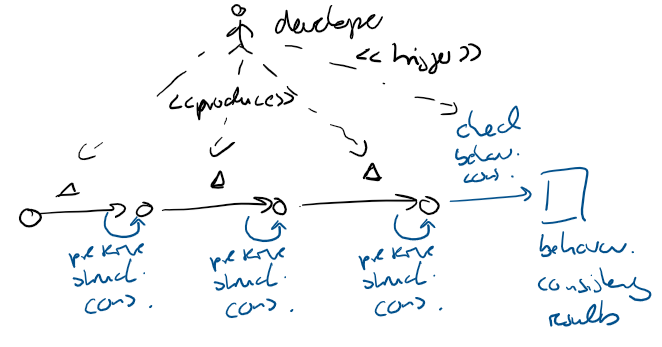
\includegraphics[width=0.8\textwidth]{figures/prologue/process_structure_behavior.png}
    \caption[Process for preserving structural and behavioral consistency]{Proposed process for continuously preserving structural and explicitly checking behavioral consistency}
    \label{fig:networks:process_structure_behavior}
\end{figure}

\mnote{Fine-grained preservation of structural relations}
In consequence, the distinction between structural and behavioral consistency relation is also relevant for the processes of checking and preserving consistency.
While structural consistency relations may be preserved often in a fine-grained way, behavioral consistency relations may be checked less often.
We depict the proposed process in \autoref{fig:networks:process_structure_behavior}.
In the best case, a consistency mechanism can give hints to potential behavioral consistency violations more often.
For example, a performance-relevant modification of the implementation could lead to a hint for the developer that performance may be affected by his modification with the information about the previous analysis result, such that he can guess whether his modification will violate the requirement.
Given the information that a response time requirement of 10 milliseconds was fulfilled during the last check by an actual response time of 1 millisecond could help the developer to decide that his modification will not violate that requirement.

\mnote{We focus on structural relations}
In this thesis, we are interested in processes that continuously preserve and not only check consistency.
This is why we explicitly focus on structural consistency relations in this thesis, although the insights might be transferable to behavioral relations as well.
As another consequence, those structural relations that we consider are supposed be decomposable into binary relations, as discussed in \autoref{chap:networks:notions:types}.



%%
%% CONSISTENCY SPECIFICATION PROCESS
%%
\section{Consistency Specification Process}
\label{chap:networks:specification_process}

\mnote{Roles and scenarios in the specification process}
In this thesis, we are concerned with the process of specifying consistency in terms of a transformation network and different problems arising in that process.
We therefore discuss which roles are involved in that process and which different scenarios can be considered that induce requirements and exemplify the application contexts of our later contributions.
\autoref{fig:networks:roles_and_process} gives an overview of the roles and the essential specification process.
While that specification process is concerned with the metamodel level (M2), a transformation network is finally applied at the model level (M1) to a concrete system under development.

\begin{figure}
    \centering
    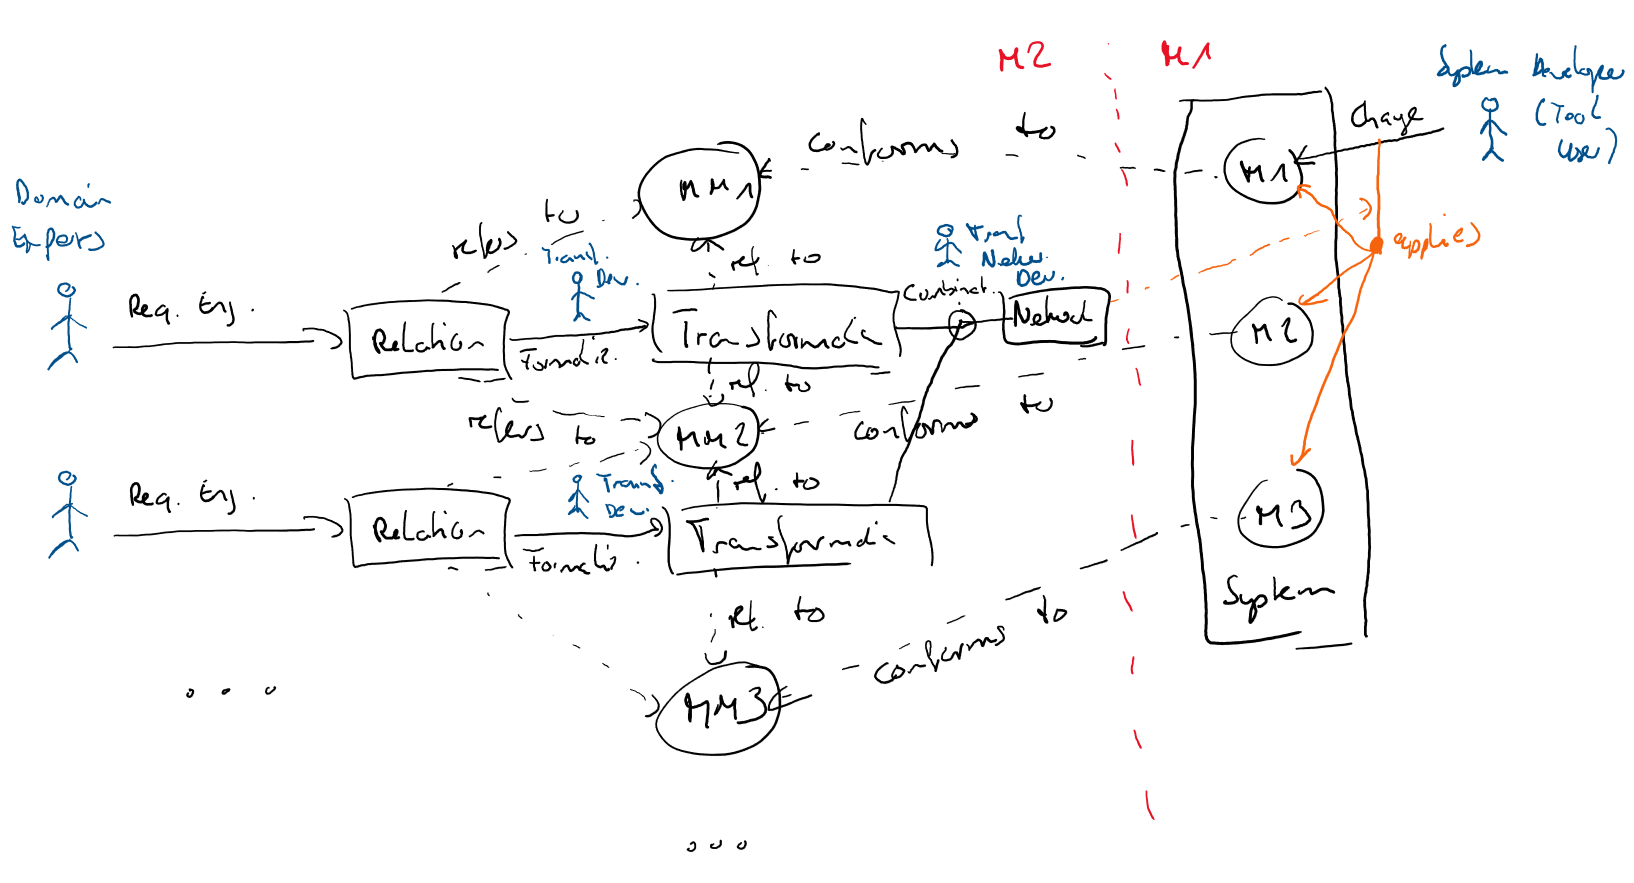
\includegraphics[width=\textwidth]{figures/prologue/networks/roles_and_process}
    \caption[Roles in a transformation network specification process]{Roles involved in a process for specifying a transformation network, their responsibilities and dependencies.}
    \label{fig:networks:roles_and_process}
\end{figure}


\subsection{Roles}

\mnote{Roles in the consistency process}
The specification of a transformation network involves the definition of the individual transformations by \emph{domain experts} and \emph{transformation developers} as well as their combination to a network by \emph{transformation network developers}.
The usage of the network, on the other hand, involves its application to changes to a system under development by a \emph{system developer}, sometimes also called \emph{tool user}~\cite{klare2019dagstuhl}.
Apart from the explicit transformation network, these roles and their responsibilities are comparable to the ones we defined in a Dagstuhl seminar~\cite{klare2019dagstuhl}.

\mnote{Roles for the specification}
A domain expert has the knowledge about the consistency relations between two (or more) tools or, more specifically, the metamodels describing them.
He performs the requirements engineering task for the information to define in a transformation.
A transformation developer is then responsible for formalizing these relations and their preserving in a transformation.
We will usually only refer to the transformation developer, as for us it is not of specific interest where the information about the relations comes from but only that it is encoded into a transformation.
Finally, a transformation network developer combines different transformations, which were usually developed by different transformation developers, to a transformation network.
It may even be possible that several transformation network developers compose several transformation networks to a larger transformation network.

\mnote{Roles for the usage}
Concrete systems are developed by system developers, which perform changes of models via the tools they use.
Thus, we also call them tool users.
Usually different system developers will be responsible for different models.
In our introductory example, we distinguished between software architects, developers, requirements engineers and so on.
Performing changes leads to the application of the transformation network to restore consistency of the models.

\mnote{Multiple roles fulfillable by same persons}
The roles reflect the different responsibilities when specifying and using transformation networks.
Several of them can, however, be fulfilled by the same persons.
This especially applies to domain experts and transformation developers.
The same person may know about the relations as a domain expert and formalize them in a transformation.
Actually the domain expert may even be the one who develops a concrete system as a system developer.



\subsection{Scenarios}

\mnote{Generic and project-specific transformations}
Both for the development of transformations, as well as for the combination of transformation to a network, different development scenarios can be distinguished.
Transformations can be developed generically or specific for a project:
\begin{properdescription}
    \item[Generic:] Transformations are developed as artifacts off-the-shelf, which can be used in any project. This especially applies for descriptive transformations (cf. \autoref{chap:networks:notions:normative_descriptive}), which only encode a common understanding of consistency, such as for \gls{UML} class models and Java code.
    \item[Project-specific:] Transformation are developed specific for a project. This can be the case, because specific rules how elements shall be related are used in a project. For example, the mapping of components to their realization in the implementation can be specific to the project. Project-specific transformation can, however, later also be used in a generic way.
\end{properdescription}

\mnote{Big bang and continuous combination of transformations}
The combination of transformations to networks can be distinguished especially regarding the point in time when the combination takes place:
\begin{properdescription}
    \item[Big bang:] Transformations are developed first and after they have been completed, a transformation network developer combines them to a network. Problems regarding the compatibility of the transformations are first recognized during this combination, thus transformations may need to be adapter afterwards to properly work together.
    \item[Continuous:] Transformations are be combined to a network already during their development. Starting with partial or even empty transformations, the structure of the network can be defined early. This allows for a continuous checking of the compatibility of the developed transformations. Ultimately, even an online checking of compatibility after each change to a transformation can be performed to get early feedback.
\end{properdescription}

\mnote{Transformation combination process affects compatibility detection}
For us, it is not relevant whether transformations are developed in a generic or project-specific way.
The distinction of scenarios in which transformation networks are developed is, however, of special interest.
It can be beneficial for transformation developers to get feedback on the compatibility of their developed transformations with others on-the-fly.
This makes locating a problem easier, because only the last changes may have induced it, whereas with an a-posteriori checking the complexity to find compatibility problems potentially increases because of missing locality.

\mnote{Processes can be mixed}
While both generic as well as project-specific transformation can be mixed in a single project, also the process of combining them may be mixed.
Some of the transformation may be integrated in a big bang fashion, whereas others are continuously integrated.
This can also be a result of where the transformation come from.
A generic transformation cannot be continuously integrated, because it is not specific for a single project to integrate it into.



%%
%% MODELS AND METAMODELS
%%
\section{Models and Metamodels}

The most essential elements throughout this thesis are models and the metamodels describing them.
We have already introduced in \autoref{chap:foundations} what we consider a model and that we adhere to the modelling formalism defined by the \gls{MOF}.
We use a sufficiently simplified notion of models, metamodels and their elements, for which we give an overview in \autoref{tab:networks:elements}.

\todo{Change the following to definitions rather than only a table}

\begin{table}
\centering
\renewcommand{\arraystretch}{1.4}%
%\rowcolors{2}{white}{gray!15}
%\setlength\tabcolsep{4 pt}
\begin{tabular}{R{4.8cm} L{5cm}}
\toprule
\multicolumn{2}{c}{Properties and Classes}\\
$P$                 
    & Property (attribute or reference) \\
$\metamodelinstances{P} = \setted{p_1, p_2, \dots}$     
    & Property values of a property $P$ \\
$\class{C}{} = \tupled{P_1, \dots, P_n}$
    & Class \\
$\metamodelinstances{C} = \setted{o = \tupled{p_1, \dots, p_n} \mid p_i \in \metamodelinstances{P_i}}$ 
    & Instances (objects) of a class $\class{C}{}$\\
$\object{o}{} \in \metamodelinstances{C}$
    & Object of a class $\class{C}{}$ \\
\midrule
\multicolumn{2}{c}{(Meta-)Models}\\
$\metamodel{M}{} = \setted{\class{C}{1}, \dots, \class{C}{m}}$
    & Metamodel\\
$\metamodelinstances{M} = \setted{m \mid m \subseteq \bigcup_{\class{C}{} \in \metamodel{M}{}} \metamodelinstances{C}}$
    & Instances of a metamodel\\
$\metamodelset{M} = \setted{\metamodel{M}{1}, \dots, \metamodel{M}{k}}$
    & Set of metamodels\\
$\metamodelinstances{\metamodelset{M}} = \setted{ \setted{\model{m}{1}, \dots, \model{m}{k}} \mid \model{m}{i} \in \metamodelinstances{\metamodel{M}{i}}}$
    & Instances of a metamodel set $\metamodelset{M}$\\
$\model{m}{} \in \metamodelinstances{M}$
    & Model of metamodel $\metamodel{M}{}$\\
$\modelset{m} \in \metamodelinstances{\metamodelset{M}}$
    & Model set of a metamodel set $\metamodelset{M}$\\
\bottomrule
\end{tabular}
\caption{Models, metamodels, their elements and notations}
\label{tab:networks:elements}
\end{table}

\subsection{Notation}

In general, we use variables of uppercase letters for all elements at the metamodel level (M2), such as $\metamodel{M}{}$ for a metamodel or $\class{C}{}$ for a class, whereas we use lowercase letters for all elements at the model level (M1), such as $\model{m}{}$ for a model and $\object{o}{}$ for an object.
If not further specified, we use the same indices on related elements on the metamodel and the model level, such as model $\model{m}{1}$ being an instance of metamodel $\metamodel{M}{1}$.

\subsection{Elements}

In general, we consider metamodels as a composition of meta-classes, which in turn are composed of properties representing attributes or references.
Models instantiate metamodels and are composed of objects, which are instances of meta-classes and in turn consist of property values, which instantiate properties.

We denote \emph{properties}, which are the information a meta-class consists of, such as attributes or references, as $P$ and the \emph{property values} as instances of a property as $\metamodelinstances{P} = \setted{p_1, p_2, \dots}$ of property $P$. 
We do not need to further differentiate different types of properties into attributes and references, like it is done in other formalizations, such as the OCL standard~\cite[A.1]{ocl} or the thesis of \citeauthor{kramer2017a}~\cite[2.3.2]{kramer2017a}.

We denote \emph{meta-classes}, in the following shortly called \emph{classes}, as tuples of properties $\class{C}{} = \tupled{P_1, \dots, P_n}$. 
Instances of a \emph{class} are \emph{objects}, each being a tuple of instances of the properties of the class and we denote all instances of a class $\class{C}{}$ as $\metamodelinstances{C} = \setted{o = \tupled{p_1, \dots, p_n} \mid p_i \in \metamodelinstances{P_i}}$.

We denote a metamodel $\metamodel{M}{} = \setted{\class{C}{1}, \dots, \class{C}{m}}$ as a finite set of classes.
The instances of a metamodel are sets of objects $\metamodelinstances{M} = \setted{m \mid m \subseteq \bigcup_{\class{C}{} \in \metamodel{M}{}} \metamodelinstances{C}}$.
Those instance sets are, in other work like~\cite{stevens2020BidirectionalTransformationLarge-SoSym} with more lightweight definitions of metamodels, sometimes also simply called \emph{model sets}.
Each instance, denoted as a \emph{model}, is a finite set of objects that instantiate the classes in the metamodel.
For a set of metamodels $\metamodelset{M} = \setted{\metamodel{M}{1}, \dots, \metamodel{M}{k}}$, we denote the set that contains all sets of instances of that metamodels as $\metamodelinstances{\metamodelset{M}} = \setted{ \setted{\model{m}{1}, \dots, \model{m}{k}} \mid \model{m}{i} \in \metamodelinstances{\metamodel{M}{i}}}$.



\subsection{Assumptions}

We assume models to be finite, so for each model $\model{m}{}$, we assume that $|\model{m}{}| < \infty$.
Additionally, our formalism assumes objects to be unique within a model $\model{m}{}$. 
This is already implicitly covered by the definition of $\metamodelinstances{M}$ for the instances of a metamodel $\metamodel{M}{}$. 
In practice, it is usually allowed to have the same object, i.e., an element with the same type, attribute and reference values, multiple times within the same model. 
This is, however, only a matter of identity, which we assume, without loss of generality, to be represented within the objects, whereas identity in practice is given by different objects being placed at specific places in memory.

% Our definition of models does not restrict validity of models apart from being a collection of instances of the classes in the metamodel.
% It is possible to define further constraints for metamodels that restrict their valid instances.
% We intentionally do not consider such restrictions of valid models, because even a single transformation 

\todoDiss{Discuss valid models, why we do not consider them and prove that invariants + consistency relations can express any consistency relation.
A single relation can consider constraints on the single models, but combination (even within one transformation) can easily contradict constraints of a model.}



%%
%% RUNNING EXAMPLE
%%
\section{Running Example}
\label{chap:networks:example}

\todo{Address von Resident in "Location" auslagern und Address von "Person" in Address auslagern. Also remove $R'_{ER}$ and move it to compatibility chapter, as it is not yet relevant here.}

\begin{figure}
    \centering
    %% From motivational_example in MPM4CPS paper

\newcommand{\hdistance}{14em}
\newcommand{\classwidth}{6em}

\begin{tikzpicture}

% Person
\umlclassvarwidth{person}{}{Person\sameheight}{
firstname\\
lastname\\
address\\
income
}{\classwidth}

% Employee
\umlclassvarwidth[,above right=2em and \hdistance of person.east, anchor=south]{employee}{}{Employee\sameheight}{
name\\
socsecnumber\\
salary
}{\classwidth}

\umlclassvarwidth[,below=4em of employee.south, anchor=north]{resident}{}{Resident\sameheight}{
name\\
address\\
socsecnumber
}{\classwidth}


% CONSISTENCY RELATIONS
\draw[consistency relation] (person.north) |- node[pos=0, above left] {$p$} node[pos=0.75, above] {$\consistencyrelation{CR}{PE}$} node[pos=1, above left] {$e$} (employee.west);
\draw[consistency relation] (employee.south) -- node[pos=0, below left] {$e$} node[right, align=left] {$\consistencyrelation{CR}{ER}$}% /\\ $R'_{ER}$} 
node[pos=1, above left] {$r$} (resident.north);
\draw[consistency relation] (resident.west) -| node[pos=0, below left] {$r$} node[pos=0.25, below] {$\consistencyrelation{CR}{PR}$} node[pos=1, below left] {$p$} (person.south);

\draw[consistency relation 2] (person.east) -- node[pos=0, below right] {$p$} ++(0.35*\hdistance,0) -- node[pos=0, above=0.5em] {$\consistencyrelation{CR}{PER}$} node[pos=1, above left] {$e$} ([yshift=1em]employee.south west);
\draw[consistency relation 2, -latex] ([xshift=0.35*\hdistance]person.east) -- node[pos=1, below left] {$r$} ([yshift=-1em]resident.north west);

\node[consistency related element 2, below left=5em and 2em of person.south west, anchor=north west, inner sep=0em] (relations1) {
$\begin{aligned}
    \consistencyrelation{CR}{PER} =\; &
            \setted{\tupled{p,e,r} \mid 
            %& 
            \mathvariable{p.firstname} + \text{\enquote{\textvisiblespace}} + \mathvariable{p.lastname} = \mathvariable{e.name} = \mathvariable{r.name} \\
            &
            \land \mathvariable{p.address} = \mathvariable{r.address}
            \land \mathvariable{p.income} = \mathvariable{e.salary} \\
            &
            \land \mathvariable{e.socsecnumber} = \mathvariable{r.socsecnumber}
        }
\end{aligned}$
};

\node[consistency related element, below=0.5em of relations1.south west, anchor=north west, inner sep=0em] {
$\begin{aligned}
    \consistencyrelation{CR}{PE} =\; &
            \setted{\tupled{p,e} \mid %\\
            %& 
            \mathvariable{p.firstname} + \text{\enquote{\textvisiblespace}} + \mathvariable{p.lastname} = \mathvariable{e.name}%\\
            %& 
            \land \mathvariable{p.income} = \mathvariable{e.salary}
        }\\[0.3em]
        \consistencyrelation{CR}{PR} =\; &
            \setted{\tupled{p,r} \mid %\\
            %& 
            \mathvariable{p.firstname} + \text{\enquote{\textvisiblespace}} + \mathvariable{p.lastname} = \mathvariable{r.name}%\\
            %& 
            \land \mathvariable{p.address} = \mathvariable{r.address}
        }\\[0.3em]
        \consistencyrelation{CR}{ER} =\; &
            \setted{\tupled{e,r} \mid %\\
            %& 
            \mathvariable{e.name} = \mathvariable{r.name} %\\
            %& 
            \land \mathvariable{e.socsecnumber} = \mathvariable{r.socsecnumber}
        }%\\
    % R'_{ER} =\; &
    %         \setted{\tupled{e,r} \mid %\\
    %         %& 
    %         e.name.toLower = r.name\\
    %         & \land e.socsecnumber = r.socsecnumber
    %     }
\end{aligned}$
};

\end{tikzpicture}
    \caption[Three metamodels with exemplary consistency relations]{Three simple metamodels for persons, employees and residents, one ternary relation $R_{PRE}$ between them and three binary relations $R_{PE}, R_{PR}, R_{ER}$ for each pair of them, with $R'_{ER}$ as an alternative for $R_{ER}$.}
    \label{fig:networks:three_persons_example}
\end{figure}

We use different variations of a running example throughout several parts of this thesis.
The basic example is depicted in \autoref{fig:prologue:three_persons_example}.
It contains three metamodels, one with persons, one with employees and one with residents.
Although these metamodels are rather simple and do not cover metamodels from the software engineering domain, they are sufficient to explain the concepts in this thesis and easy to comprehend.

The example also contains a description of consistency between these three metamodels, although only informally given and more precisely defined later on.
It requires that if any person, employee or resident is contained in a model, there must also be the other two elements with the same names, addresses, incomes and social security numbers.
This relation can either be expressed as a ternary relation, denoted as $R_{PER}$, or as three binary relations $R_{PE}, R_{PR}, R_{ER}$.



% \begin{copiedFrom}{ICMT}
    
% % EXEMPLARY PROBLEMS
% Consider the simple consistency relations exemplified in \autoref{fig:properties:motivational_example}.
% A company uses three software systems to manage (1)~personnel data, (2)~tasks and their assignment to employees, and (3)~schedules for work times of employees and the deadlines of tasks.
% The domain models contain dependent information, especially the data about employees and their relations to tasks, but none of them contains a superset of information of another, which requires to define consistency between all pairs of them.
% If three domain experts define %the consistency constraints between all pairs of the metamodels 
% those binary constraints
% independently, they can easily contradict. 
% For example, imagine %that they specify 
% a direct mapping of employee \emph{name} representations between the task management and scheduling system, a concatenation of \emph{firstname} and \emph{lastname} between personnel data and task management system and a comma-separated concatenation of \emph{lastname} and \emph{firstname} between personnel data and scheduling system.
% These constraints are obviously incompatible, as they cannot be fulfilled at the same time.
% %Additionally, even if the name mappings were compatible, specifying three transformations between all pairs of metamodels that preserve those constraints leads to redundancies within the transformations.
% %In consequence, the transformation have to ensure that they no element duplications arise from that.
% %%leads to redundant the operationalization of transformations that preserve these constraints has to ensure that no element duplications arise from redundant transformations paths. 
% %%Additionally, even if the name mapping was compatible, the operationalization of transformations that preserve these constraints has to ensure that no element duplications arise from redundant transformations paths. 
% %For example, after adding an employee to the personnel data system, a transformation adds an employee to the task management system, which is then transformed into an employee in the scheduling system. 
% %The additional transformation between personnel and scheduling system must correctly consider that an employee was already created transitively.
% %\todoHeiko{Checken, ob auf Duplizierungsproblem später verwiesen wird, dann hier wieder einfügen}

% \begin{figure}[tb]
%     \centering
%     %\includegraphics[angle=270, width=\textwidth]{figures/motivation_employee_example.pdf}
%     \newcommand{\hdistance}{10.5em}
\newcommand{\classwidth}{4.5em}
\newcommand{\sameheight}{\vphantom{Êy}}

\begin{tikzpicture}

% \node[uml class] (personal_employee) {Employee
% \nodepart{two}
% name\\
% address\\
% salary\\
% dailyWorkingTime\\
% department
% };

% PERSONNEL
\umlclassvarwidth{personnel_employee}{}{Employee\sameheight}{
firstname\\
lastname\\
%address\\
salary\\
workingTime\\
department
}{\classwidth}

\node[above=0.2em of personnel_employee.north] (personnel_label) {\small \emph{(1) Personnel Data}};


% TASK MANAGEMENT
\umlclassvarwidth[,right=\hdistance of personnel_employee.north, anchor=north]{task_task}{}{Task\sameheight}{
name\\
description\\
%department
}{\classwidth}

\umlclassvarwidth[,below=1.5em of task_task.south, anchor=north]{task_employee}{}{Employee\sameheight}{
name\\
department
}{\classwidth}

\umlassociationfromto{(task_employee) -- %node[uml role end] {assigned to} 
node[uml cardinality end, pos=0.7, left] {*} node[uml role end, pos=0.65, right] {responsible for}  node[uml cardinality start, pos=0.2, left] {*} (task_task)}

\node[above=0.2em of task_task.north] (task_label) {\small \emph{(2) Task Management}};


% SCHEDULING
\umlclassvarwidth[,right=\hdistance of task_task.north, anchor=north]{scheduling_task}{}{Task\sameheight}{
name\\
deadline
}{\classwidth}

\umlclassvarwidth[,right=8.5em of scheduling_task.north, anchor=north]{scheduling_schedule}{}{Schedule\sameheight}{}{\classwidth}

\umlclassvarwidth[,below=1.5em of scheduling_schedule.south, anchor=north]{scheduling_workday}{}{WorkDay\sameheight}{
date
}{\classwidth}

\umlclassvarwidth[,right=\hdistance of task_employee.north, anchor=north]{scheduling_employee}{}{Employee\sameheight}{
name\\
workingTime
}{\classwidth}

\umlcomposition{(scheduling_schedule) -- node[uml cardinality end] {*} (scheduling_schedule-|scheduling_task.east)}
\umlcomposition{(scheduling_schedule) -- node[uml cardinality end] {*} (scheduling_workday)}
\umlassociationfromto{([yshift=-0.5em]scheduling_workday.west) -- node[uml cardinality end] {*} node[uml role end, above, pos=0.5] {working} ([yshift=-0.5em]scheduling_workday.west-|scheduling_employee.east)}
\umlassociationfromto{(scheduling_employee) -- node[uml cardinality start, pos=0.2, right] {*} node[uml cardinality end, pos=0.7, right] {*} node[uml role end, left, pos=0.6] {responsible for} (scheduling_task)}

\coordinate (scheduling_upper_middle) at ($(scheduling_schedule.north)!0.5!(scheduling_task.north)$);
\node[above=0.2em of scheduling_upper_middle] (scheduling_label) {\small \emph{(3) Scheduling}};


% CONSISTENCY RELATIONS
\draw[consistencyrel] ([xshift=0.5em]personnel_employee) |- node[pos=0.75, below, align=center] {(first/last)name,\\ department} ([yshift=-2.2em]task_employee.north west);
\draw[consistencyrel] ([yshift=-2.2em]task_employee.north east) -- node[below, align=center] {name, \\ relation to task} ([yshift=-2.2em]scheduling_employee.north west);
\draw[consistencyrel] ([xshift=-0.5em]personnel_employee.south) -- ++(0,-4.2em) -| node[above, pos=0.25] {(first/last)name, workingTime} (scheduling_employee.south);
\draw[consistencyrel] (task_task.east) -- node[below] {name} (task_task.east-|scheduling_task.west);

\end{tikzpicture}
%     %\caption{Exemplary Consistency Relations between a PCM, UML Class and Java Model}
%     \caption{Exemplary Consistency Relations ({\protect\tikz[baseline=-0.5ex] \protect\draw[latex-latex, consistency related element] (0,0) -- (1.5em,0);}) between Three Simple Metamodels} %Personnel, Task Management and Scheduling System Metamodels}
%     \label{fig:properties:motivational_example}
% \end{figure}

% % ABSTRACT PROBLEMS
% While such a problem may be trivially solvable in this simple scenario, it gets difficult in systems with more and larger metamodels, %, especially in software development or system engineering scenarios, in which 
% where
% each domain expert only knows about the relation between two of them, but not about the others.
% In consequence, each \ac{BX} has to be constructed in such a way that it can be combined with other, independently developed \acp{BX} in a \emph{black-box} manner later on.
% Issues that arise from such a combination of independently developed \acp{BX} %the combination of independently developed \acp{BX} %to networks of them 
% have not been investigated yet. %and categorized yet.
% In consequence, potential failures, causal mistakes and techniques to avoid them by design are not systematically known.

% \end{copiedFrom} % ICMT

